\documentclass[a4paper, 11pt]{article}
\usepackage{comment} 
\usepackage{fullpage} 
\usepackage{hyperref}
\usepackage{amsmath}
\usepackage{graphicx}

\usepackage{booktabs} 


\usepackage{algorithm}
\usepackage{algpseudocode}

\begin{document}
\noindent
\large\textbf{PROBLEM 3--Algorithm Selection}\hfill \textbf{Dhruviben Modi} \\
\normalsize SOEN 6011 \hfill \textbf{40166396} \\
 SOFTWARE ENGINEERING PROCESSES \hfill Due Date: August 5, 2022 \\
\hfill Github address : git@github.com:mdhruvi/SOEN-6011-project.git

\section{Gamma function with Lanczos}

\begin{algorithm}
\caption{Lanczos approximation for Gamma Function}

\textbf{Require:}  value: $x > 0$ \Comment{$x \in Z^{+}$} \\
\textbf{Ensure:} g is a constant that chosen randomly with the condition that  $ Re(z) > \frac{1}{2}$.

\begin{algorithmic}[1]

\Procedure {lanczosGamma}{x}
    \If x $< \frac{1}{2}$ then
    \State  $\Gamma (x)={\pi  \over \sin \pi x \Gamma (1-x)}$ \Comment{Reflection formula}
    \EndIf
    \State g $\leftarrow$  a small random integer
    \State P $\leftarrow$ a convergence of nine to ten terms \Comment{double floating-point precision.}
    
    
    \For {$i \leftarrow 1, P.length $}
    \State $P_{g}(x)=P_{0}+{\frac  {P_{i}}{x+i}}$
    \EndFor
    \State ${\displaystyle \Gamma (x+1)={\sqrt {2\pi }}{\left(x+g+{\tfrac {1}{2}}\right)}^{x+{\frac {1}{2}}}e^{-\left(x+g+{\frac {1}{2}}\right)}P_{g}(x)}$
    
    \State \textbf{return} $\Gamma (x)$
    \EndProcedure
\Statex

\State $result \leftarrow \Gamma (x)$ 

\end{algorithmic}
\end{algorithm}

Lanczos approximation is a method for computing the gamma function numerically, It is a practical alternative to the Stirling's approximation for calculating the gamma function with fixed precision.. The Lanczos approximation extends the factorial technique, which will be used to calculate input smaller than $0.5$, by using the reflection formula. It will apply a different formula for any other values. In order to compute the gamma function with standard single or double floating-point precision and select a fixed constant g, 9 to 10 terms of the series in an aggregate are required. These terms will all be used to determine the coefficients then incorporate it into the given formula ${\displaystyle \Gamma (x+1)={\sqrt {2\pi }}{\left(x+g+{\tfrac {1}{2}}\right)}^{x+{\frac {1}{2}}}e^{-\left(x+g+{\frac {1}{2}}\right)}P_{g}(x)}$.

\section{Gamma function with Stirling}

Stirling's estimate gives an approximate value for the factorial function n! or the gamma function $\Gamma(n)$ when $n>1$. For all positive integers, ${\displaystyle n!=\Gamma (n+1)}$ is applied. The approximation can most simply be derived for n an integer by approximating the sum over the terms of the factorial with an integral, so that ${\displaystyle \ln n! = n \ln(n) - n + \Theta \ln(n)}$. However  the gamma function, unlike the factorial, is more broadly defined for all complex numbers other than non-positive integers; nevertheless, Stirling's formula may still be applied. If $Re(x) > 0$ then, specifying the constant in $\mathcal{O}(\ln(n))$ error term gives $\frac{1}{2}\ln(2\pi n)$, yielding the more precise formula $n! \sim \sqrt {2\pi n} (\frac{n}{e})^n$. Stirling's approximation can be extended to the double inequality as follow $\sqrt {2\pi n} (\frac{n}{e})^n  e^\frac{1}{12n + 1} < n! < \sqrt {2\pi n} (\frac{n}{e})^n  e^\frac{1}{12n}$ 

\begin{algorithm}

\caption{Stirling's approximation for Gamma function}

\textbf{Require:}  value: $x > 0$ \Comment{$x \in Z^{+}$}\\
\textbf{Ensure:} x is large in absolute value
\begin{algorithmic}[1]

\Procedure {stirlingGamma}{x}
    \State \indent $\Gamma (x) = \Call{squareroot}{n}$  \Comment{formula is an asymptotic expansion}
    
    \State \textbf{return} $\Gamma (x)$
    
    \Procedure{squareRoot}{n}
    \State error $\leftarrow$ 0.00001
    \State errorPrecision $\leftarrow$ 1
    \State temp $\leftarrow$ n
    \While {$errorPrecision > error$}
        \State $n \leftarrow \frac{{n}+ \frac{temp}{n}}{2}$
        \State $errorPrecision \leftarrow n - \frac{temp}{n}$
    \EndWhile
    \State \textbf{return} $n$
    \EndProcedure
    
    \Procedure{Power}{$base, exponent$}
    \State Convert the exponent into String
    \State $exponentArray \leftarrow Split\; the\; exponent\; into\; integer\; and\; fractional\; part $
    \If {$exponentArray[1] > 0$} 
     \State \qquad \textbf{return} $\Call{fractionPower}{base, exponent}$ \Comment{it returns fractionPower}
     \EndIf
     \If {$ exponent < 0$} 
     \State \qquad $base \leftarrow 1/base$
     \State \qquad $exponent \leftarrow exponent * (-1)$
     \State \textbf{return} \Call{power}{base, exponent} \Comment{it returns the power}
     \EndIf
     \State else if $exponent \leftarrow 0$ then
     \State \qquad \textbf{return} 1 \Comment{it returns 1}
     \State else if  $exponent \mod  2 \leftarrow 0$ then 
     \State \qquad $base \leftarrow base * base $
     \State \qquad $exponent \leftarrow exponent/2 $
     \State \textbf{return} \Call{exponent}{base , exponent} \Comment{it returns power}
     \State else
     \State \qquad $exponent \leftarrow (exponent-1)/2$
     \State \textbf{return}\; $base$ * \Call{power}{base * base , exponent} \Comment{it returns the power}
    \EndProcedure

\EndProcedure
\end{algorithmic}
\end{algorithm}

\begin{algorithm}
\begin{algorithmic}[1]
    \Procedure{stirlingGamma}{x}
    \Procedure{fractionPower}{$base, exponent$}
    \If {$exponent \leftarrow 0$}
    \State \qquad \textbf{return} 1.0  \Comment{it returns the value 1}
    \EndIf
    \If {$base < 0$} 
    \State \qquad $ln \leftarrow \Call{logarithm}{base * (-1)}$
    \EndIf
    \State else
    \State \qquad $ln \leftarrow \Call{logarithm}{base}$
    \If {$base \leftarrow 0$ and $exponent > 0$} 
    \State \qquad \textbf{return} answer \Comment{it returns the answer}
    \EndIf
    \For{$i \leftarrow 1, 125$}
    \State \qquad $u \leftarrow \Call{power}{exponent*ln , i}$
    \State \qquad $l \leftarrow \Call{factorial}{i}$
    \State \qquad answer = answer + (u/l)
    \EndFor 
    \If {$base < 0\;  $and$\;  exponent\;$ mod\; 2$ \neq  0$} 
    \State \qquad \textbf{return} $answer * (-1)$ \Comment{it returns the answer * (-1)}
    \EndIf
    \State else
    \State \qquad \textbf{return} answer; \Comment{it returns the answer}
    \EndProcedure
    
    \Procedure{logarithm}{n}
    \State $base \leftarrow (n - 1) / (n + 1)$
    \For{$i \leftarrow 1, 125$} 
    \State \qquad  $e \leftarrow {2*i-1}$
    \State \qquad $r \leftarrow {r+(1/e) * \Call{power}{base, exponent}}$
    \EndFor
    \State \textbf{return} 2 * $r$ \Comment{it returns a}
    \EndProcedure
    
    \Procedure{factorial}{$n$}
    \State \qquad \textbf{return}   \Call{factorialtailRecursion}{n,1} \Comment{it returns recursivefactorial function}
    \EndProcedure
    
    \Procedure{factorialtailRecusrion}{$n, a$}
    \If {$n \leftarrow 0$} 
    \State \qquad \textbf{return} a;\Comment{it returns a}
    \EndIf
    \State \textbf{return} \Call{factorialTailRecursive}{n-1 , n*a}\Comment{it returns factorialTailRecursive }
    \EndProcedure
    \EndProcedure
\Statex

\State $result \leftarrow \Gamma (x)$
\end{algorithmic}
\end{algorithm}


\newpage
\section{Advantages And Disadvantages}
\subsection{ The Lanczos approximation method}
\begin{itemize}
    \item{Performance : Evidently, the Lanczos approximation method increases efficiency compared to the original gamma function defined simply as ${\displaystyle \Gamma (x)=\int _{0}^{\infty }t^{x-1}e^{-t}\,dt}$ which need the integral calculating.}
    
    \item{Area of Application: Compared to the regular factorial function, which can only handle positive integers, the Lanczos approximation approach for the gamma function provides a wider range of applications. The method can be extended over the complete complex plane without the negative integer using the reflection formula, but it is only valid for arguments in the right complex half-plane when using the formula deduction.}
    
    \item{Accurateness : The outcome deviates slightly since the Lanczos approach is still only an approximation.}
    
    \item{Disadvantages : It can be challenging to calculate the Lanczos coefficients, and how well the calculations turn out relies on the two arbitrary parameters, g and n. Another disadvantage is that for fixed real parts of the free parameter, utilising complex coefficients increases calculation time while decreasing accuracy of the Lanczos approximation.}
\end{itemize} 

\subsection{ The Stirling's approximation method}
\begin{itemize}
    \item{Performance : Since it takes time to resolve convergent improper integration, the Stirling's approximation method is more efficient than the original gamma function.}
    
    \item{Area of Application: For any complex numbers other than non-positive integers, the Stirling's approximation for gamma function is more generally defined than the factorial, but Stirling's approximation can still be used.}
    
    \item{Accurateness : The benefit of the Stirling approximation approach is that even when the value of the parameter x is relatively small, the result is still quite accurate and results are almost identical when the value of the parameter x is large.}

    \item{Disadvantage : The drawback of this approach cannot comprehend real values that are less than or equal to $0$.}
\end{itemize}

\subsection{Conclusion}
The Stirling's approximation method is quite straightforward when compared to other gamma function implementation techniques.

\newpage
\section{MindMap}

\begin{figure}[h]
    \centering
    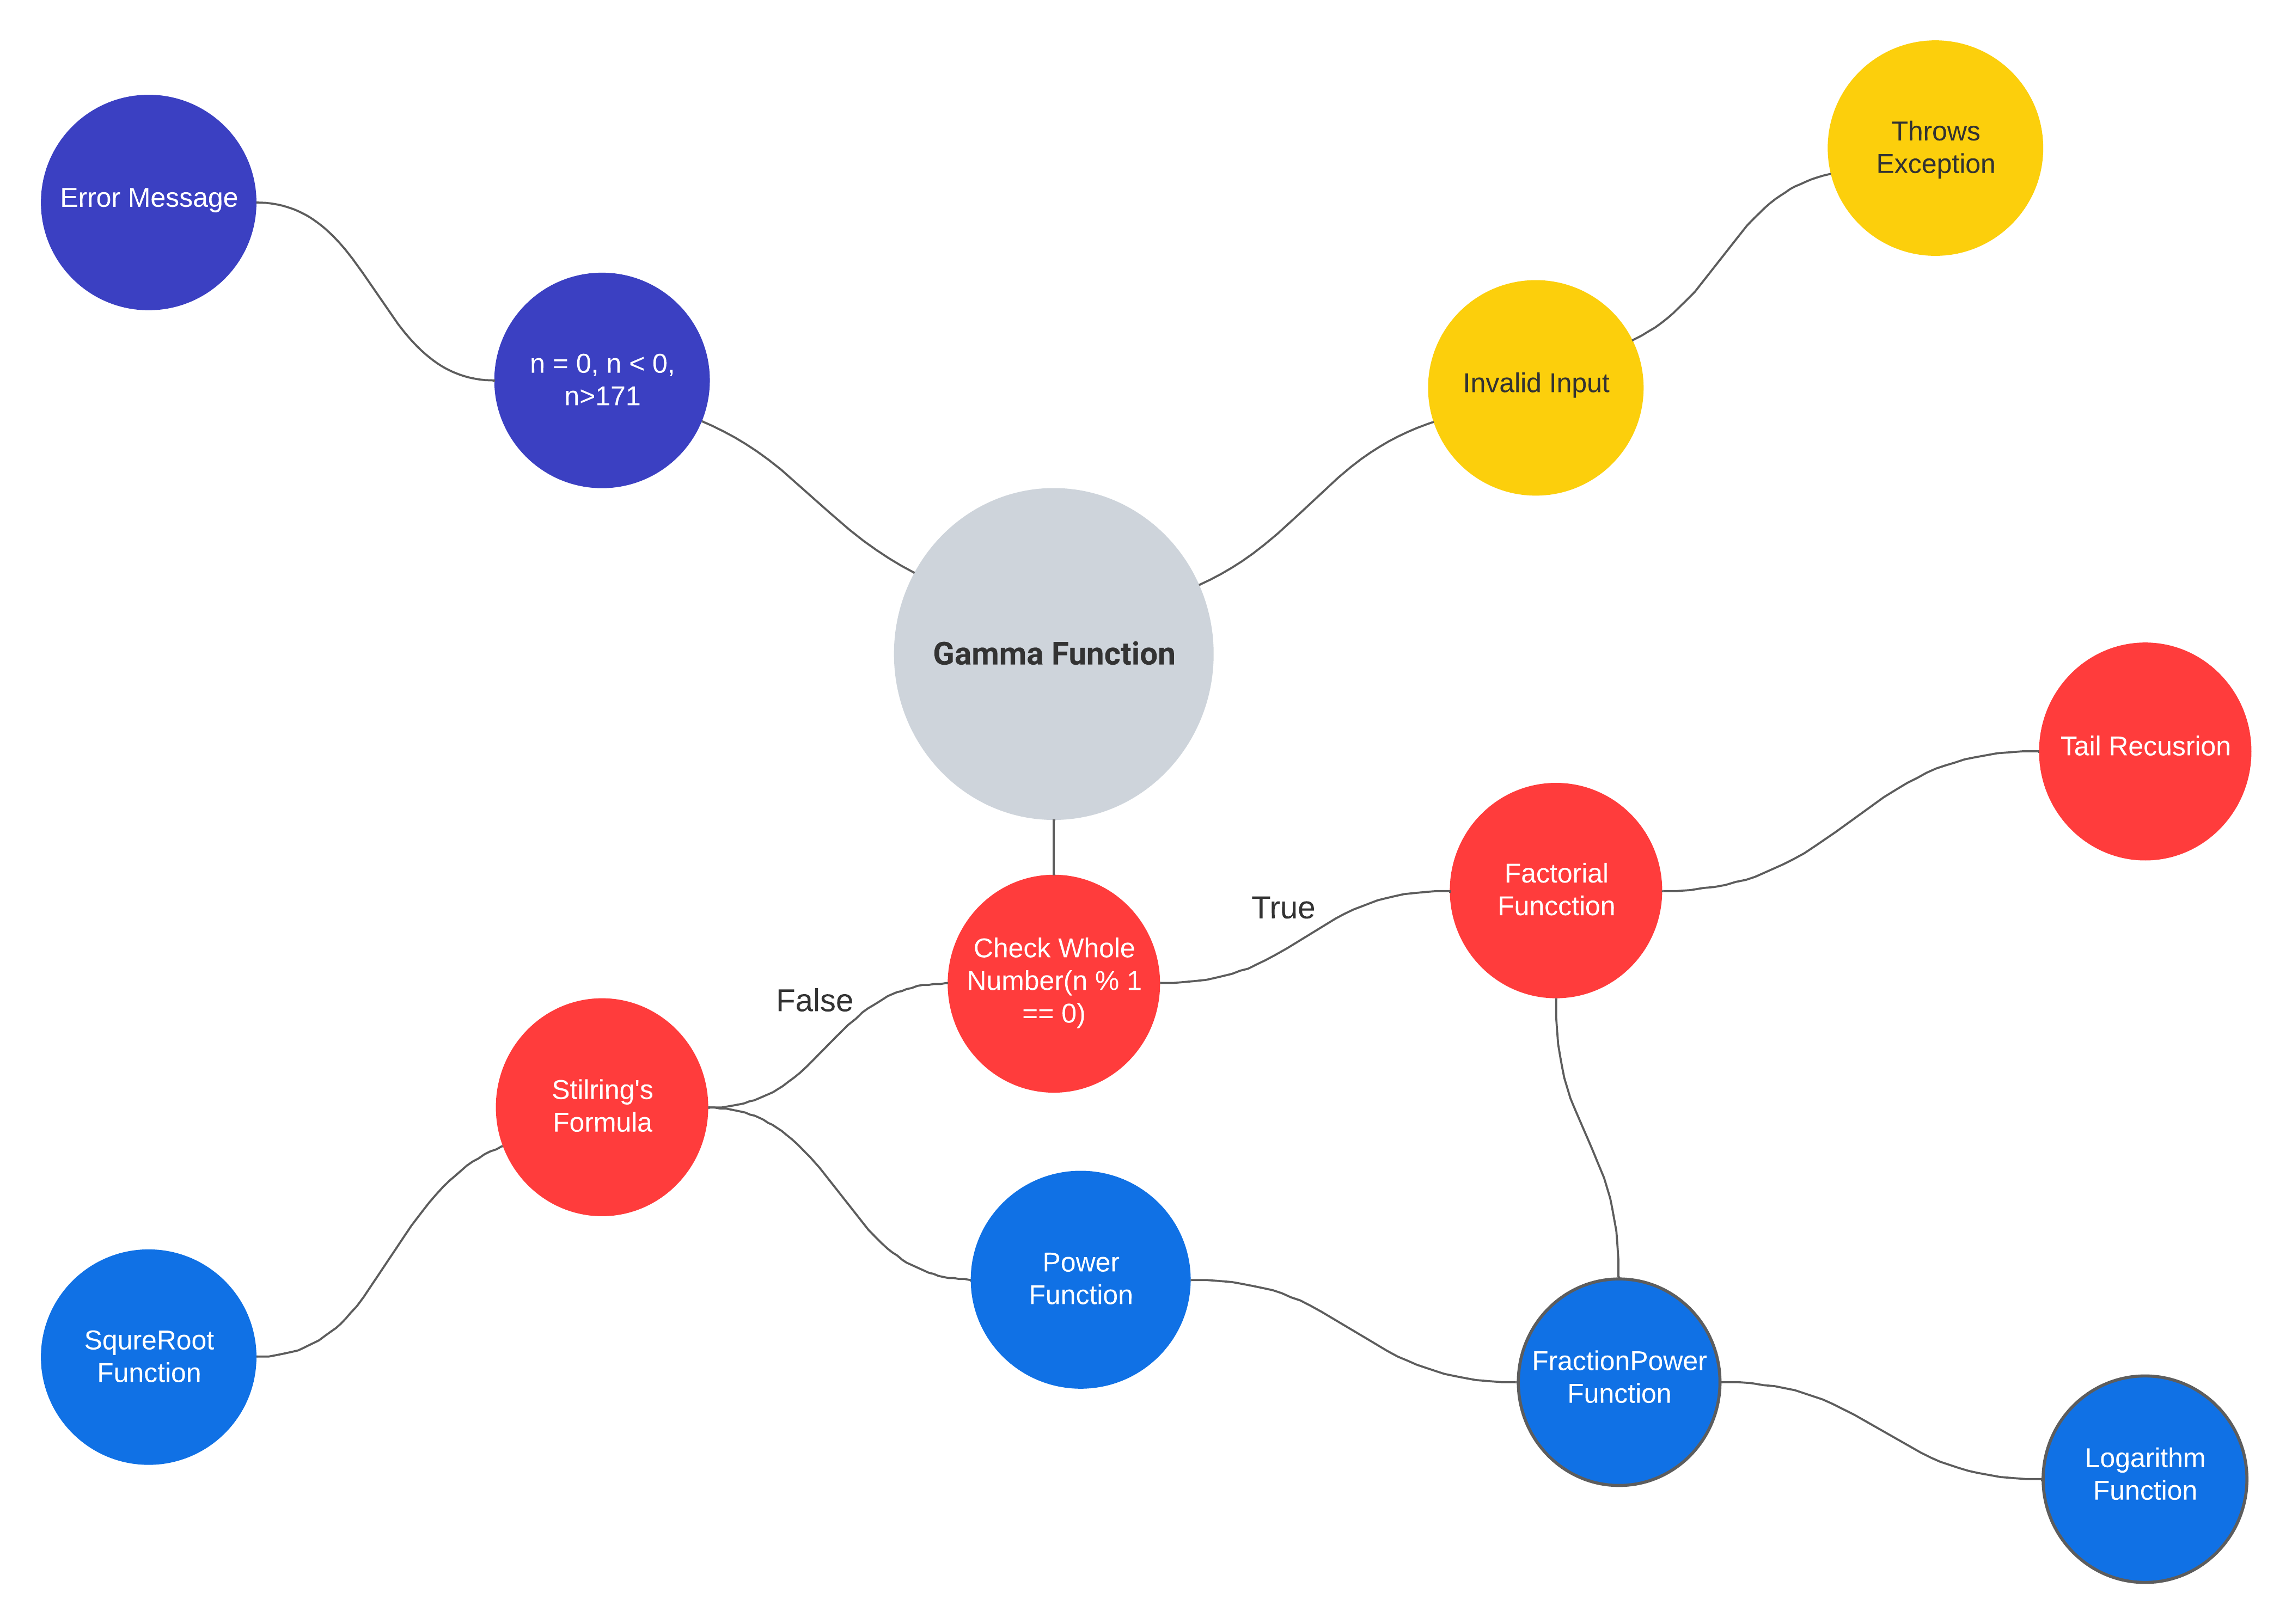
\includegraphics[width=1.0\linewidth]{Images/Mind map.png}
    \caption{MindMap to implement Gamma Function.}
    \label{fig:Exp_Data}
\end{figure}

\section{References}
Stirling's Formula.
https://mathworld.wolfram.com/StirlingsApproximation.html\\

\noindent
Stirling's approximation. (2019, May 18). Retrieved from https://en.wikipedia.org/wiki/Stirling's-approximation-An-alternative-derivation \\

\noindent
Lanczos approximation.(2019, June 25). Retrieved from https://en.wikipedia.org/wiki/Lanczos-approximation
\end{document}